% Options for packages loaded elsewhere
\PassOptionsToPackage{unicode}{hyperref}
\PassOptionsToPackage{hyphens}{url}
%
\documentclass[
]{book}
\usepackage{amsmath,amssymb}
\usepackage{lmodern}
\usepackage{iftex}
\ifPDFTeX
  \usepackage[T1]{fontenc}
  \usepackage[utf8]{inputenc}
  \usepackage{textcomp} % provide euro and other symbols
\else % if luatex or xetex
  \usepackage{unicode-math}
  \defaultfontfeatures{Scale=MatchLowercase}
  \defaultfontfeatures[\rmfamily]{Ligatures=TeX,Scale=1}
\fi
% Use upquote if available, for straight quotes in verbatim environments
\IfFileExists{upquote.sty}{\usepackage{upquote}}{}
\IfFileExists{microtype.sty}{% use microtype if available
  \usepackage[]{microtype}
  \UseMicrotypeSet[protrusion]{basicmath} % disable protrusion for tt fonts
}{}
\makeatletter
\@ifundefined{KOMAClassName}{% if non-KOMA class
  \IfFileExists{parskip.sty}{%
    \usepackage{parskip}
  }{% else
    \setlength{\parindent}{0pt}
    \setlength{\parskip}{6pt plus 2pt minus 1pt}}
}{% if KOMA class
  \KOMAoptions{parskip=half}}
\makeatother
\usepackage{xcolor}
\IfFileExists{xurl.sty}{\usepackage{xurl}}{} % add URL line breaks if available
\IfFileExists{bookmark.sty}{\usepackage{bookmark}}{\usepackage{hyperref}}
\hypersetup{
  pdftitle={AFSC Fishery Stock Assessment SOP},
  pdfauthor={alphabetical and Ben Williams},
  hidelinks,
  pdfcreator={LaTeX via pandoc}}
\urlstyle{same} % disable monospaced font for URLs
\usepackage{color}
\usepackage{fancyvrb}
\newcommand{\VerbBar}{|}
\newcommand{\VERB}{\Verb[commandchars=\\\{\}]}
\DefineVerbatimEnvironment{Highlighting}{Verbatim}{commandchars=\\\{\}}
% Add ',fontsize=\small' for more characters per line
\usepackage{framed}
\definecolor{shadecolor}{RGB}{248,248,248}
\newenvironment{Shaded}{\begin{snugshade}}{\end{snugshade}}
\newcommand{\AlertTok}[1]{\textcolor[rgb]{0.94,0.16,0.16}{#1}}
\newcommand{\AnnotationTok}[1]{\textcolor[rgb]{0.56,0.35,0.01}{\textbf{\textit{#1}}}}
\newcommand{\AttributeTok}[1]{\textcolor[rgb]{0.77,0.63,0.00}{#1}}
\newcommand{\BaseNTok}[1]{\textcolor[rgb]{0.00,0.00,0.81}{#1}}
\newcommand{\BuiltInTok}[1]{#1}
\newcommand{\CharTok}[1]{\textcolor[rgb]{0.31,0.60,0.02}{#1}}
\newcommand{\CommentTok}[1]{\textcolor[rgb]{0.56,0.35,0.01}{\textit{#1}}}
\newcommand{\CommentVarTok}[1]{\textcolor[rgb]{0.56,0.35,0.01}{\textbf{\textit{#1}}}}
\newcommand{\ConstantTok}[1]{\textcolor[rgb]{0.00,0.00,0.00}{#1}}
\newcommand{\ControlFlowTok}[1]{\textcolor[rgb]{0.13,0.29,0.53}{\textbf{#1}}}
\newcommand{\DataTypeTok}[1]{\textcolor[rgb]{0.13,0.29,0.53}{#1}}
\newcommand{\DecValTok}[1]{\textcolor[rgb]{0.00,0.00,0.81}{#1}}
\newcommand{\DocumentationTok}[1]{\textcolor[rgb]{0.56,0.35,0.01}{\textbf{\textit{#1}}}}
\newcommand{\ErrorTok}[1]{\textcolor[rgb]{0.64,0.00,0.00}{\textbf{#1}}}
\newcommand{\ExtensionTok}[1]{#1}
\newcommand{\FloatTok}[1]{\textcolor[rgb]{0.00,0.00,0.81}{#1}}
\newcommand{\FunctionTok}[1]{\textcolor[rgb]{0.00,0.00,0.00}{#1}}
\newcommand{\ImportTok}[1]{#1}
\newcommand{\InformationTok}[1]{\textcolor[rgb]{0.56,0.35,0.01}{\textbf{\textit{#1}}}}
\newcommand{\KeywordTok}[1]{\textcolor[rgb]{0.13,0.29,0.53}{\textbf{#1}}}
\newcommand{\NormalTok}[1]{#1}
\newcommand{\OperatorTok}[1]{\textcolor[rgb]{0.81,0.36,0.00}{\textbf{#1}}}
\newcommand{\OtherTok}[1]{\textcolor[rgb]{0.56,0.35,0.01}{#1}}
\newcommand{\PreprocessorTok}[1]{\textcolor[rgb]{0.56,0.35,0.01}{\textit{#1}}}
\newcommand{\RegionMarkerTok}[1]{#1}
\newcommand{\SpecialCharTok}[1]{\textcolor[rgb]{0.00,0.00,0.00}{#1}}
\newcommand{\SpecialStringTok}[1]{\textcolor[rgb]{0.31,0.60,0.02}{#1}}
\newcommand{\StringTok}[1]{\textcolor[rgb]{0.31,0.60,0.02}{#1}}
\newcommand{\VariableTok}[1]{\textcolor[rgb]{0.00,0.00,0.00}{#1}}
\newcommand{\VerbatimStringTok}[1]{\textcolor[rgb]{0.31,0.60,0.02}{#1}}
\newcommand{\WarningTok}[1]{\textcolor[rgb]{0.56,0.35,0.01}{\textbf{\textit{#1}}}}
\usepackage{longtable,booktabs,array}
\usepackage{calc} % for calculating minipage widths
% Correct order of tables after \paragraph or \subparagraph
\usepackage{etoolbox}
\makeatletter
\patchcmd\longtable{\par}{\if@noskipsec\mbox{}\fi\par}{}{}
\makeatother
% Allow footnotes in longtable head/foot
\IfFileExists{footnotehyper.sty}{\usepackage{footnotehyper}}{\usepackage{footnote}}
\makesavenoteenv{longtable}
\usepackage{graphicx}
\makeatletter
\def\maxwidth{\ifdim\Gin@nat@width>\linewidth\linewidth\else\Gin@nat@width\fi}
\def\maxheight{\ifdim\Gin@nat@height>\textheight\textheight\else\Gin@nat@height\fi}
\makeatother
% Scale images if necessary, so that they will not overflow the page
% margins by default, and it is still possible to overwrite the defaults
% using explicit options in \includegraphics[width, height, ...]{}
\setkeys{Gin}{width=\maxwidth,height=\maxheight,keepaspectratio}
% Set default figure placement to htbp
\makeatletter
\def\fps@figure{htbp}
\makeatother
\setlength{\emergencystretch}{3em} % prevent overfull lines
\providecommand{\tightlist}{%
  \setlength{\itemsep}{0pt}\setlength{\parskip}{0pt}}
\setcounter{secnumdepth}{5}
\usepackage{booktabs}
\usepackage{graphicx}
\usepackage{multirow}
\usepackage{adjustbox}
\ifLuaTeX
  \usepackage{selnolig}  % disable illegal ligatures
\fi
\usepackage[]{natbib}
\bibliographystyle{plainnat}

\title{AFSC Fishery Stock Assessment SOP}
\author{alphabetical and Ben Williams}
\date{2022-05-27}

\begin{document}
\maketitle

{
\setcounter{tocdepth}{1}
\tableofcontents
}
\begin{verbatim}
## here() starts at C:/Users/Ben.Williams/Work/code/afsc/sop
\end{verbatim}

\hypertarget{welcome}{%
\chapter{Welcome}\label{welcome}}

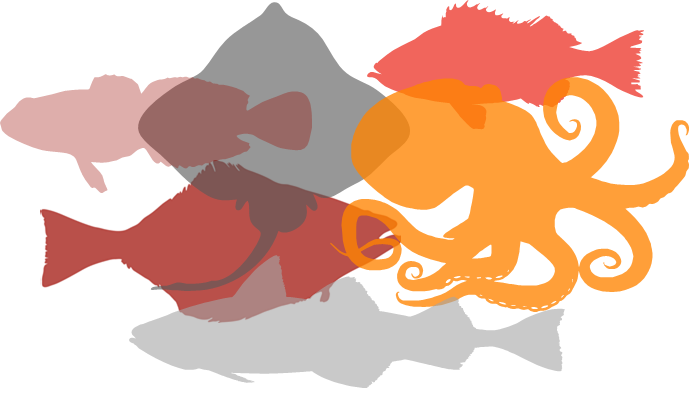
\includegraphics{images/cover.png}

The content for this book was developed as part of our group's participation in the \href{https://openscapes.org}{Openscapes Champions program}.

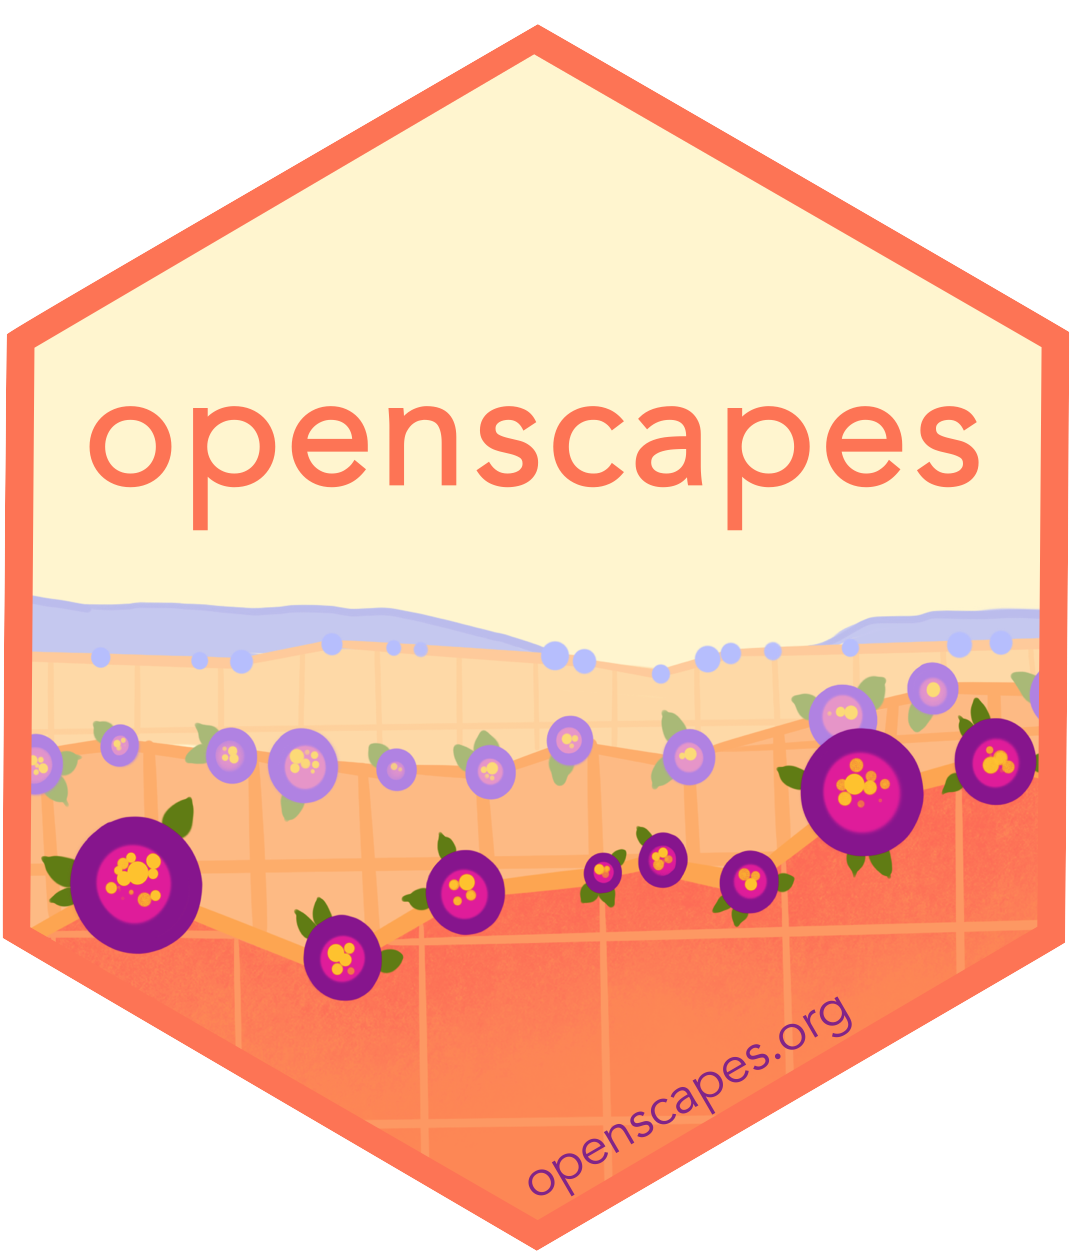
\includegraphics[width=0.25\linewidth]{images/openscapes_hex_badge}

← link to this book's GitHub repository.

If you have anything you would like to add or see something that needs corrected please create an \href{https://github.com/afsc-assessments/sop/issues}{Issue and let us know}!

\hypertarget{onboarding}{%
\chapter{Onboarding}\label{onboarding}}

\hypertarget{code-of-conduct}{%
\section{Code of conduct}\label{code-of-conduct}}

\hypertarget{git-and-github}{%
\section{Git and GitHub}\label{git-and-github}}

\hypertarget{afsc-best-practices}{%
\section{AFSC Best Practices}\label{afsc-best-practices}}

\hypertarget{file-directory}{%
\subsection{File directory}\label{file-directory}}

\hypertarget{coding-style-guide}{%
\subsection{Coding style guide}\label{coding-style-guide}}

\hypertarget{data}{%
\chapter{Data}\label{data}}

\hypertarget{getting-access}{%
\section{Getting access}\label{getting-access}}

\emph{This section was pretty much put together by Jordan Watson, thanks Jordan!!}

There are two databases in particular that you'll want access to. ``AFSC'' and ``AKFIN''. AKFIN is the Alaska Fisheries Information Network (our version of ACCSP).
These are both Oracle databases but require different logins and different network connections.
To get an AFSC account, your supervisor will need to submit a helpdesk request.
To get an AKFIN account, you will need to contact Bob Ryznar at Pacific States Marine Fisheries Commission (\href{mailto:RRyznar@psmfc.org}{\nolinkurl{RRyznar@psmfc.org}}).
With Bob, specify that you'd like access via both Answers (online GUI) and SQL (it's two different accounts).

Before getting your accounts, you will need to get on the ``signer's list'' which gives you access to confidential data.
Sign both the federal and state ones which will give you full access to most things in AKFIN (including fish tickets).
Contact Obren Davis at the AKRO to get the paperwork.
This will not give you access to VMS data. That's a separate process.

\textbf{CRITICAL:} If you mess up your password in the AFSC database 3 times, your account is locked and you need the admin to reset you. Seriously.
It's a pain.
You have to change your password every three months. Easy to change in \texttt{sql\ developer}.

\textbf{Recommended:} have IT load \texttt{SQLDeveloper} on computer.

todo: add examples of changing in sql developer

You will need to have IT install the Oracle odbc driver.
Take the code chunks below (AFSC and AKFIN) and copy and paste them into a blank text document and save that document as \texttt{tnsnames.ora}.
Give this \texttt{.ora} file to the IT person when they are setting up your account.

\begin{verbatim}
afsc =
  (DESCRIPTION =
    (ADDRESS = (PROTOCOL = TCP)(HOST = raja.afsc.noaa.gov)(PORT = 1521))
    (CONNECT_DATA =
      (SERVER = DEDICATED)
      (SERVICE_NAME = afscp1)
    )
  )

akfin =
  (DESCRIPTION =
    (ADDRESS = (PROTOCOL = TCP)(HOST = akfindb.psmfc.org)(PORT = 2045))
    (CONNECT_DATA =
      (SERVER = DEDICATED)
      (SERVICE_NAME = akfin.psmfc.org)
    )
  )
\end{verbatim}

Some simple terminology for when you are communicating with the AKFIN folks. ``AKFIN'' is the database. The schema is essentially like a folder and inside of it are all the tables.

\hypertarget{passwords}{%
\section{Passwords}\label{passwords}}

Your AFSC database password expires every 90 days.
Fortunately it is easy to update using Oracle SQL Developer.

Step 1. Open Oracle SQL Developer\\
Step 2. Right click the AFSC connection, then click on ``Reset Password''.

\begin{Shaded}
\begin{Highlighting}[]
\NormalTok{knitr}\SpecialCharTok{::}\FunctionTok{include\_graphics}\NormalTok{(here}\SpecialCharTok{::}\FunctionTok{here}\NormalTok{(}\StringTok{\textquotesingle{}figs\textquotesingle{}}\NormalTok{, }\StringTok{\textquotesingle{}pwd1.png\textquotesingle{}}\NormalTok{))}
\end{Highlighting}
\end{Shaded}

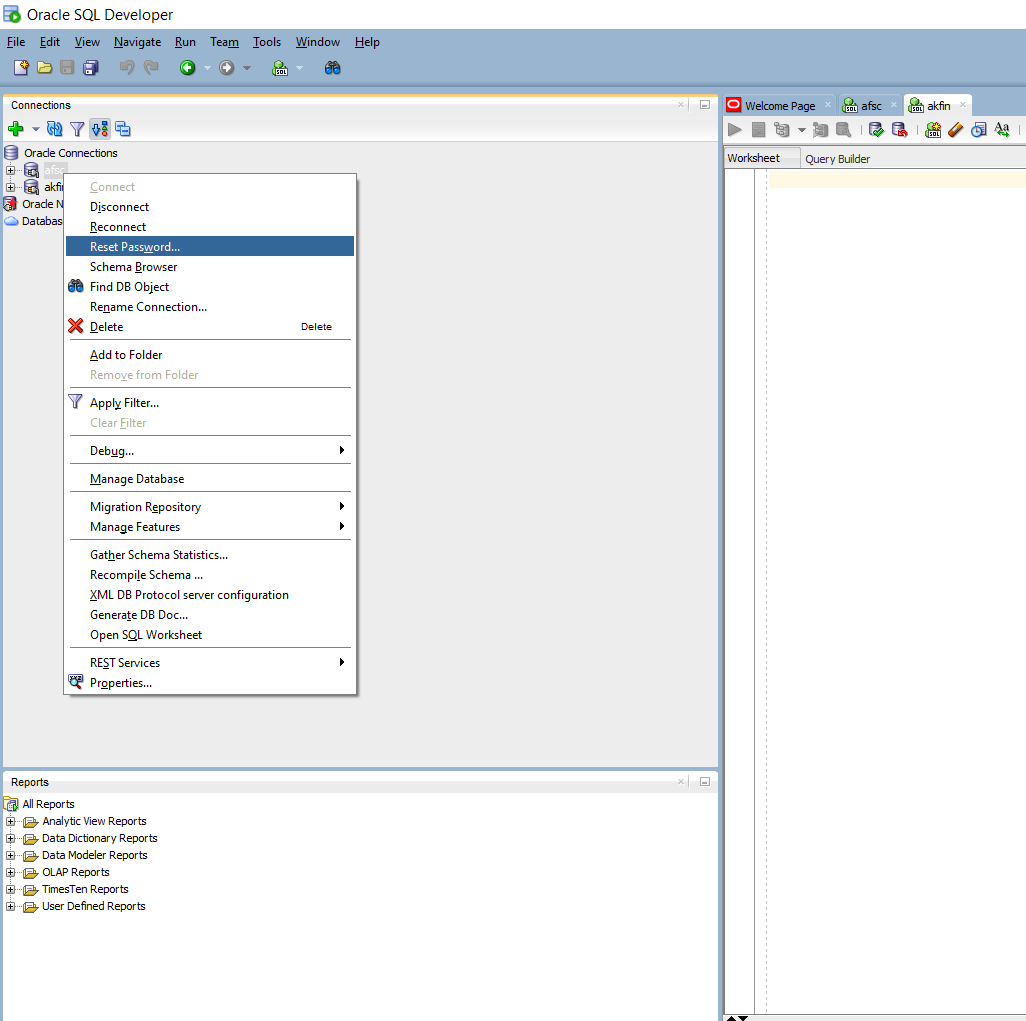
\includegraphics{figs/pwd1.png}

\hypertarget{confidentiality}{%
\section{Confidentiality}\label{confidentiality}}

Some data we just aren't permitted to share\ldots{}

\hypertarget{handling-confidential-data-on-github}{%
\subsection{Handling confidential data on GitHub}\label{handling-confidential-data-on-github}}

\hypertarget{easy-method}{%
\subsubsection{Easy method}\label{easy-method}}

Use \texttt{.gitignore} and keep any confidential files from being pushed to github.

\hypertarget{local-commit-but-not-yet-pushed-to-github}{%
\subsubsection{Local commit but not yet pushed to GitHUb}\label{local-commit-but-not-yet-pushed-to-github}}

In this scenario you have accidentally \textbf{committed the wrong files} to Git, \textbf{but haven't pushed the commit to GitHub}.
There are several ways to ``undo'' a series of commits.
The method you choose depends upon the desired outcome:

\begin{itemize}
\tightlist
\item
  Undo commit and keep all files staged: \texttt{git\ reset\ -\/-soft\ HEAD\^{}}
\item
  Undo commit and unstage all files: \texttt{git\ reset\ HEAD\^{}}

  \begin{itemize}
  \tightlist
  \item
    Undo last 3 commits and unstage all files: \texttt{git\ reset\ HEAD\textasciitilde{}3}
  \end{itemize}
\item
  Undo the commit and completely remove all changes: \texttt{git\ reset\ -\/-hard\ HEAD\^{}}
\end{itemize}

Generally speaking you will want to use \texttt{git\ reset\ HEAD\^{}}.

\includegraphics{https://www.cloudsavvyit.com/p/uploads/2021/07/f5026f58.png?trim=1,1\&bg-color=000\&pad=1,1}

\hypertarget{accidentally-pushed-to-github}{%
\subsubsection{Accidentally pushed to GitHUb}\label{accidentally-pushed-to-github}}

\hypertarget{crab-data}{%
\section{Crab data}\label{crab-data}}

\hypertarget{groundfish-data}{%
\section{Groundfish data}\label{groundfish-data}}

\hypertarget{bering-sea}{%
\subsection{Bering Sea}\label{bering-sea}}

Stratum numbers in the AKFIN tables designate different levels of data grouping.
These designations are different for the different surveys (EBS slope vs EBS shelf).
Given that these groupings are made at different levels, care should be taken not to sum values over all strata because this can duplicate data.

\hypertarget{ebs-slope-stratum-designations}{%
\subsubsection{EBS SLOPE STRATUM DESIGNATIONS:}\label{ebs-slope-stratum-designations}}

Strata include (\texttt{1:6,\ 11:15,\ 21:25,\ 31:35,\ 41:45,\ 5:55,\ 61:65,\ 999999}).

For 1-digit ``strata'', the digit designates the Canyons ordered 1 - 6 , south to north, as follows:

\begin{itemize}
\tightlist
\item
  \texttt{1\ -\ Bering\ Canyon}
\item
  \texttt{2\ -\ Pribilof\ Canyon}
\item
  \texttt{3\ -\ Inter\ Pribilof-Zhemchug}
\item
  \texttt{4\ -\ Zhemchug\ Canyon}
\item
  \texttt{5\ -\ Inter\ Zhemchug-Pervenets}
\item
  \texttt{6\ -\ Navarin/Pervenets\ Canyons}
\end{itemize}

For 2-digit ``strata'', the 1st digit designates the slope Canyon as above, and the 2nd digit designates the depth zone grouped into 200 m ranges as follows:

2nd digit:

\begin{itemize}
\tightlist
\item
  \texttt{200-400\ m} depth zone
\item
  \texttt{400-600\ m} depth zone
\item
  \texttt{600-800\ m} depth zone
\item
  \texttt{800-1000\ m}depth zone
\item
  \texttt{1000-1200\ m} depth zone
\end{itemize}

Thus, for example:

Stratum \texttt{1} = Bering Canyon, all depths within that Canyon\\
Stratum \texttt{2} = Pribilof Canyon, all depths within that Canyon\\
Stratum \texttt{11} = Bering Canyon at depths of 200-400 m\\
Stratum \texttt{65} = Navarin/Pervenets Canyons at depths of 1000-1200 m

Finally, there is a combined overall Stratum designation:
\texttt{999999} = all Canyons over all depth zones

Thus, biomass for \texttt{stratum=999999} is the same as the sum of biomass for strata \texttt{1+2+3+4+5+6}, or the sum of biomass for strata (\texttt{11+12+13+14+15+21+22+23+24+25+31+32+33+34+35+41+42+43+44+45+51+52+53+54+55+61+62+63+64+65}).

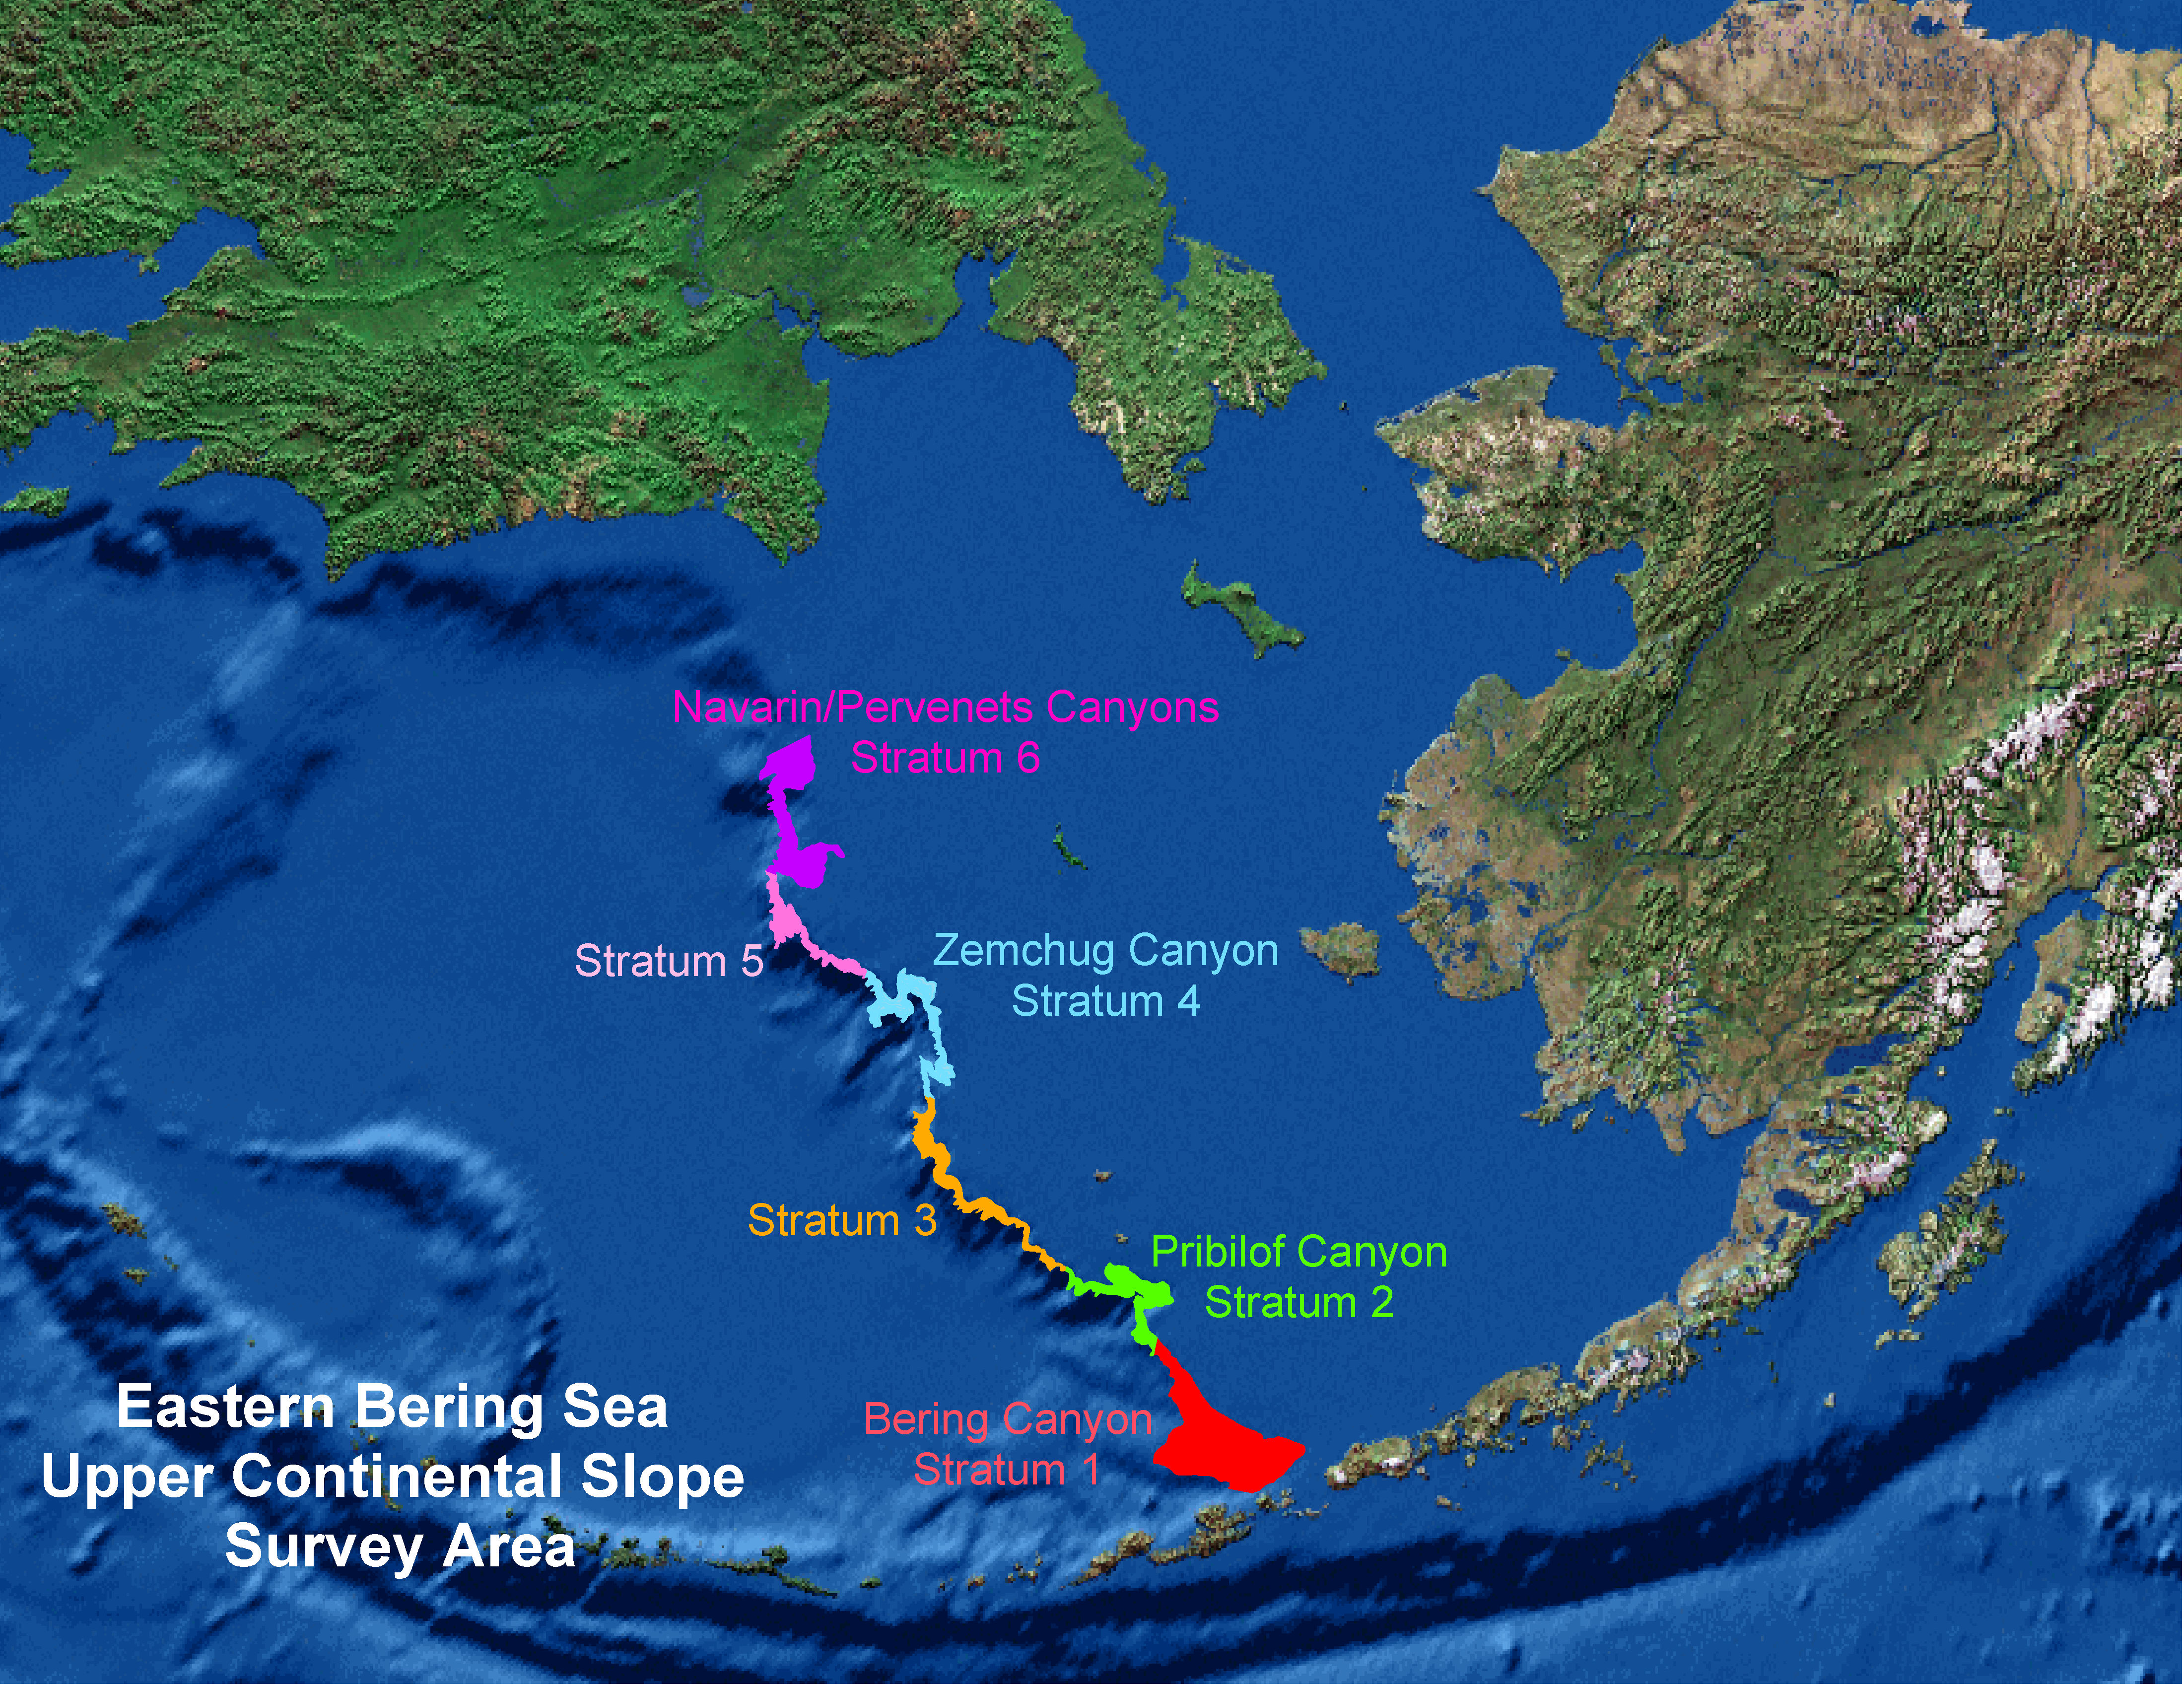
\includegraphics[width=800px,height=460px]{figs/EBS_slope_strata}

\hypertarget{ebs-shelf-stratum-designations}{%
\subsubsection{EBS SHELF STRATUM DESIGNATIONS:}\label{ebs-shelf-stratum-designations}}

Strata include (\texttt{1:10,\ 20,\ 31,\ 32,\ 41:43,\ 50,\ 61,\ 62,\ 82,\ 90,\ 100,\ 200,\ 300,\ 999}).

Please refer to the stratum map for location of strata.
Strata \texttt{10,\ 20,\ 31,\ 32,\ 41,\ 42,\ 43,\ 50,\ 61,\ 62,\ 82,\ 90} are the core strata within which biomass and population are computed.
The other strata (\texttt{1:9,\ 100,\ 200,\ 300,\ 999}) are various summations of the core strata, as follows:

\begin{itemize}
\tightlist
\item
  \texttt{10}
\item
  \texttt{20}
\item
  \texttt{31+32}
\item
  \texttt{41+42+43}
\item
  \texttt{50}
\item
  \texttt{61+62}
\item
  \texttt{82}
\item
  \texttt{90}
\end{itemize}

\texttt{100} = depth zone \textless50 m (=strata 1+2; or 10+20)\\
\texttt{200} = depth zone 50-100 m (=strata 3+4+8; or 31+32+41+42+43+82)\\
\texttt{300} = depth zone 100-200 m (=strata 5+6+9; or 50+61+90)

\texttt{999} = overall combined (all strata = \texttt{1+2+3+4+5+6+8+9}; or \texttt{10+20+31+32+41+42+43+50+61+62+82+90})

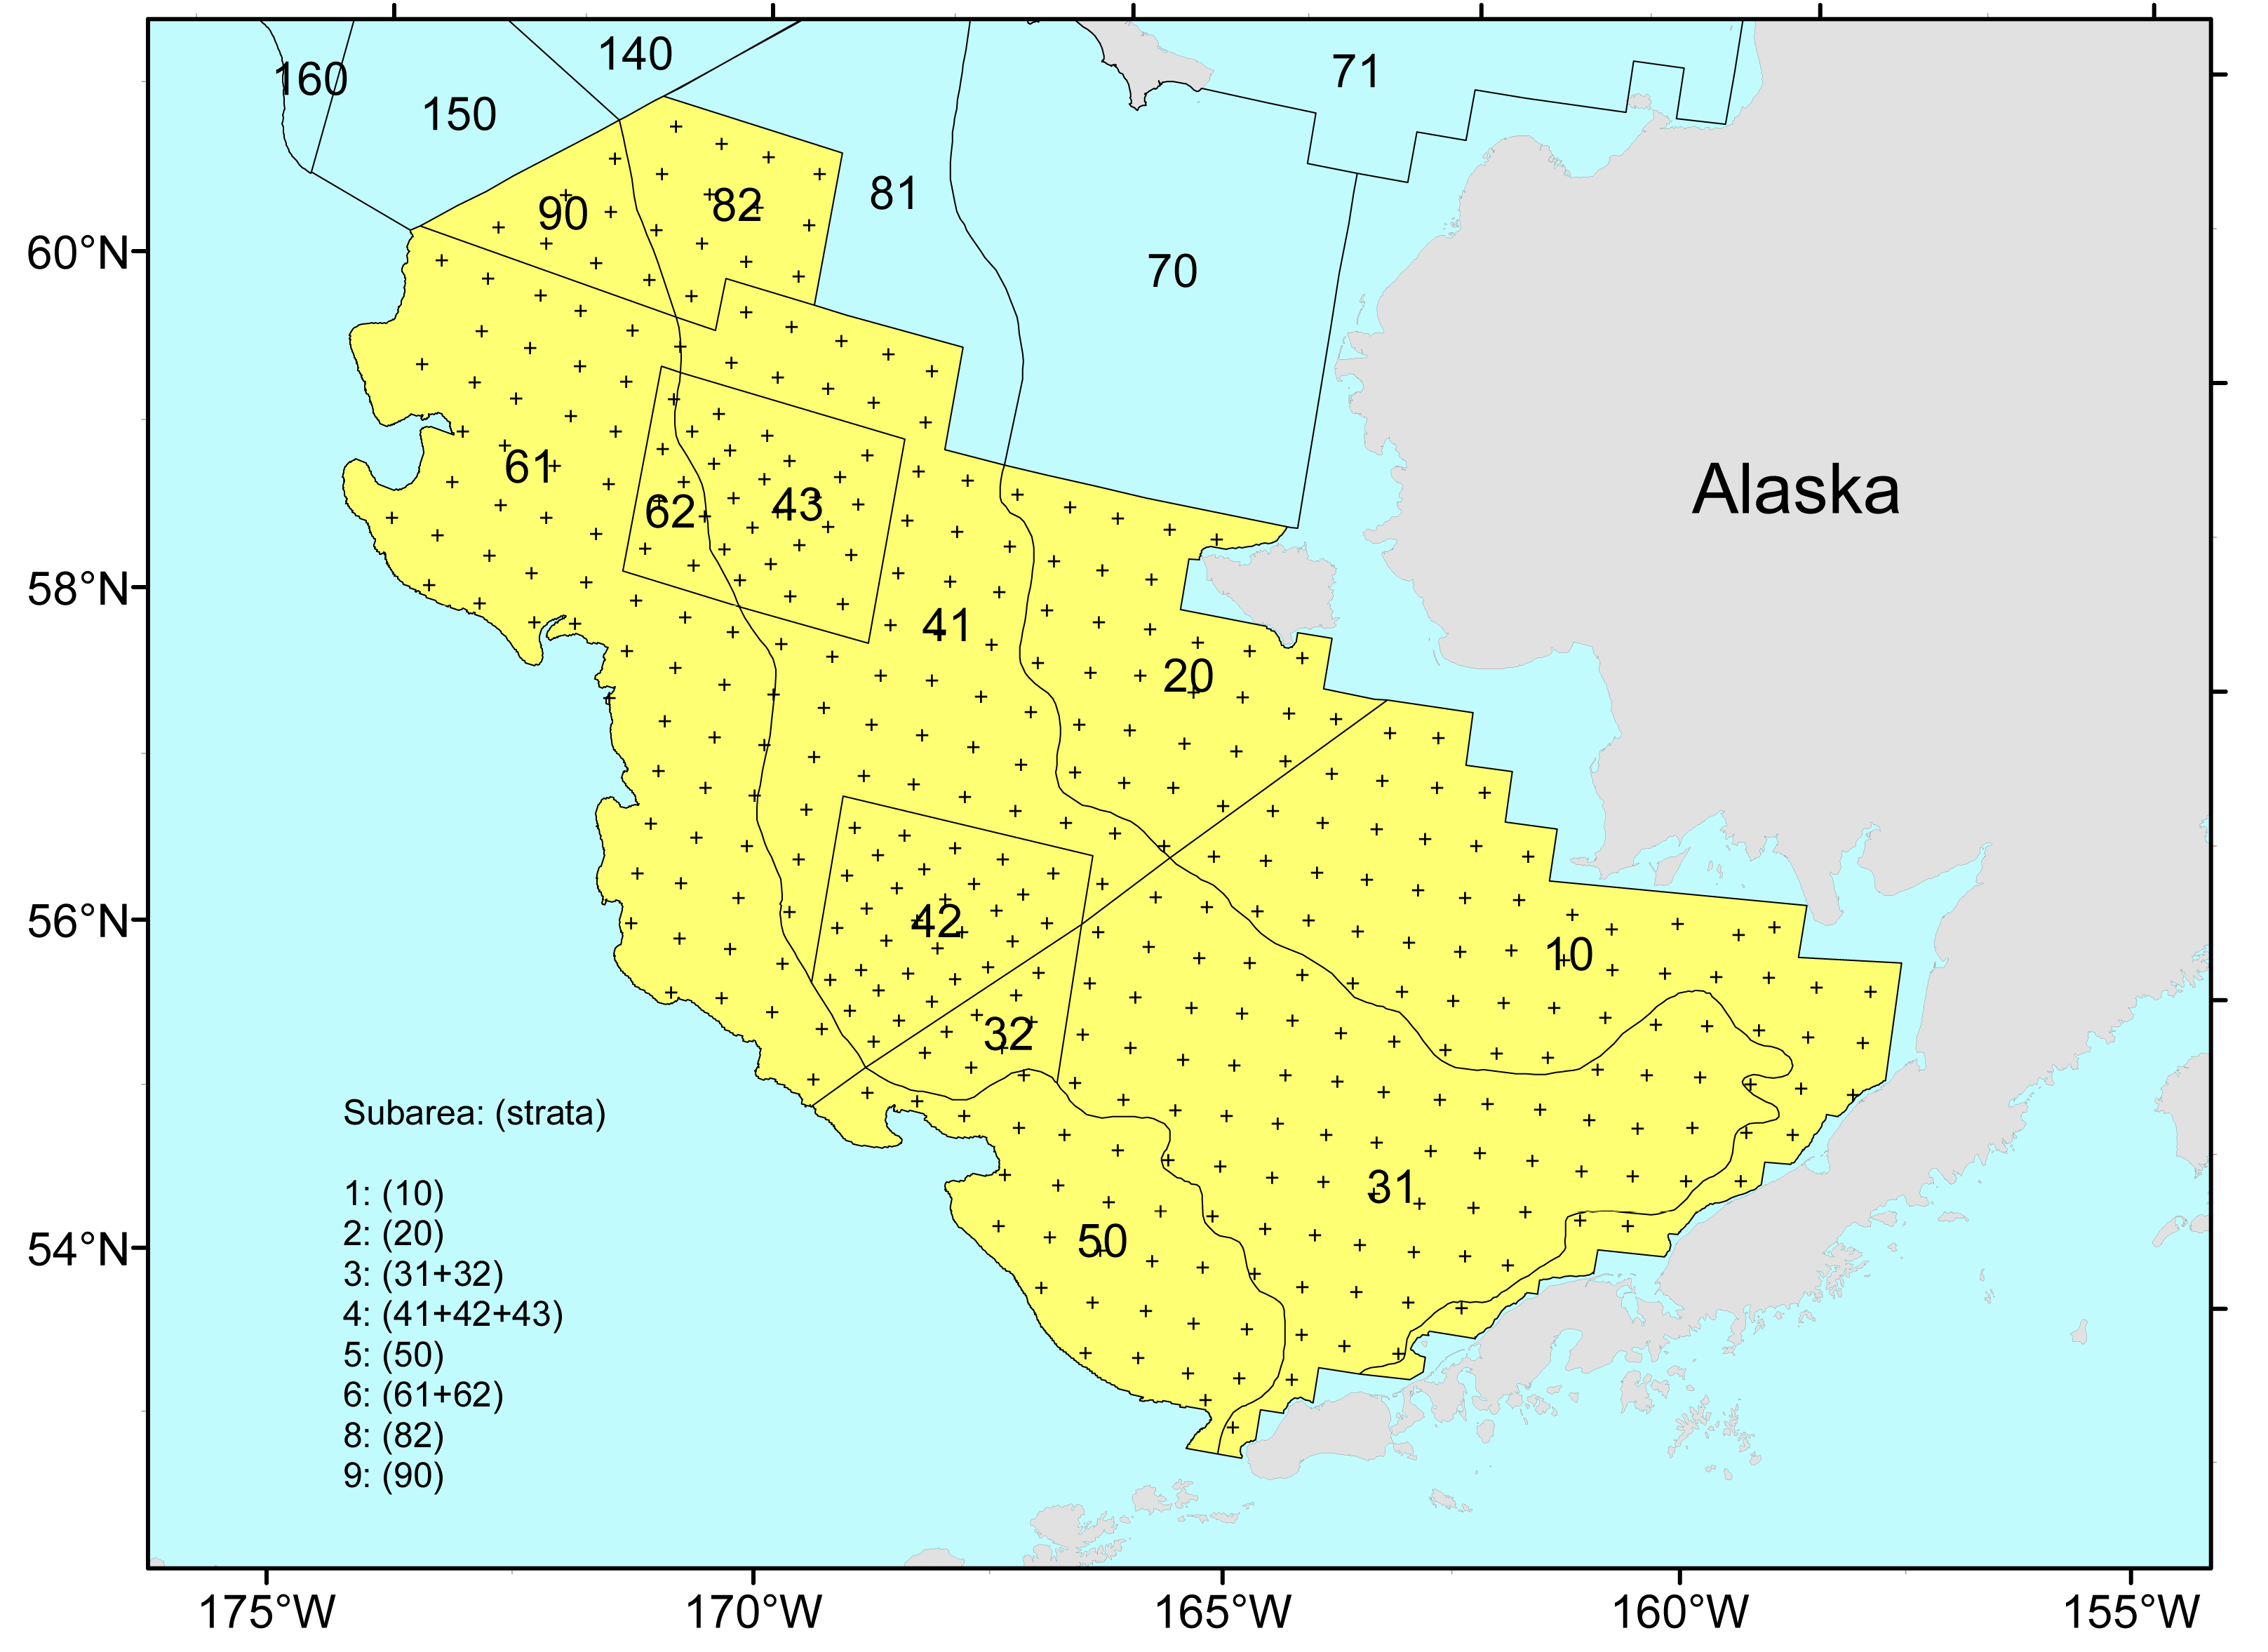
\includegraphics[width=800px,height=460px]{figs/EBS_shelf_strata}

\hypertarget{aleutian-islands}{%
\subsection{Aleutian Islands}\label{aleutian-islands}}

\hypertarget{gulf-of-alaska}{%
\subsection{Gulf of Alaska}\label{gulf-of-alaska}}

\hypertarget{safe}{%
\chapter{Crab SAFE Guidelines}\label{safe}}

I have no idea!!

\hypertarget{groundfish-safe-guidelines}{%
\chapter{Groundfish SAFE Guidelines}\label{groundfish-safe-guidelines}}

Need to have AFSC google drive access for this:
\href{https://docs.google.com/document/d/1ykEGhbvwY7iKRTclUHb-hCObHLoWW6g2dF-pwb85_1o/edit\#heading=h.gjdgxs}{Safe guidelines}

  \bibliography{book.bib,packages.bib}

\end{document}
